% -*- TeX-master: "main"; fill-column: 72 -*-

\section{Proposed syntax and semantics}
\label{syntax}

In this section, we define the syntax and semantics of the Flux Balance
Constraints package for SBML Level~3 Version~1.  We expound on the various
data types and constructs defined in this package, then in \sect{examples},
we provide complete examples of using the constructs in an example SBML
model.

\subsection{Namespace URI and other declarations necessary for using this
package}
\label{xml-namespace}

Every SBML Level~3 package is identified uniquely by an XML namespace URI.
For an SBML document to be able to use a given SBML Level~3 package, it
must declare the use of that package by referencing its URI.  The following
is the namespace URI for this version of the Flux Balance Constraints
package for SBML Level~3 Version~1:
\begin{center}
\texttt{http://www.sbml.org/sbml/level3/version1/fbc/version3}
\end{center}


In addition, SBML documents using a given package must indicate whether
understanding the package is required for complete mathematical interpretation
of a model, or whether the package is optional.  This is done using the
attribute \token{required} on the \token{<sbml>} element in the SBML document.
For the \FBCPackage, the value of this attribute must be set to \val{false}.

The following fragment illustrates the beginning of a typical SBML model
using SBML Level~3 Version~1 and this version of the Flux Balance
Constraints package:

\begin{example}
<?xml version="1.0" encoding="UTF-8"?>
<sbml xmlns="http://www.sbml.org/sbml/level3/version1/core" level="3" version="1"
   xmlns:fbc="http://www.sbml.org/sbml/level3/version1/fbc/version3" fbc:required="false">
\end{example}

\begin{figure}[ht!]
  \centering
  % Requires \usepackage{graphicx}
  %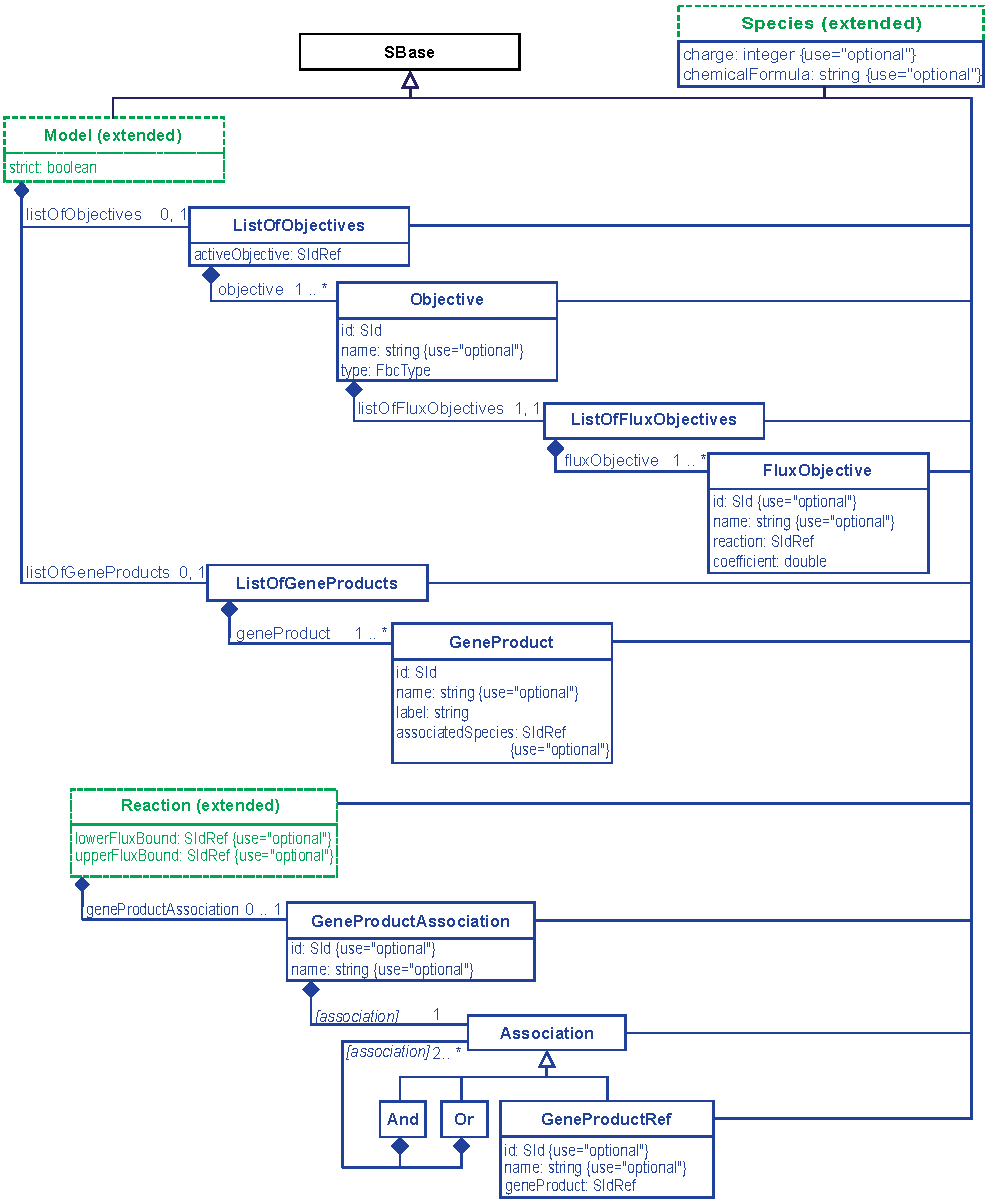
\includegraphics[width=0.85\textwidth]{images/v3harmony_fbc_uml.pdf}\\
  %V3
  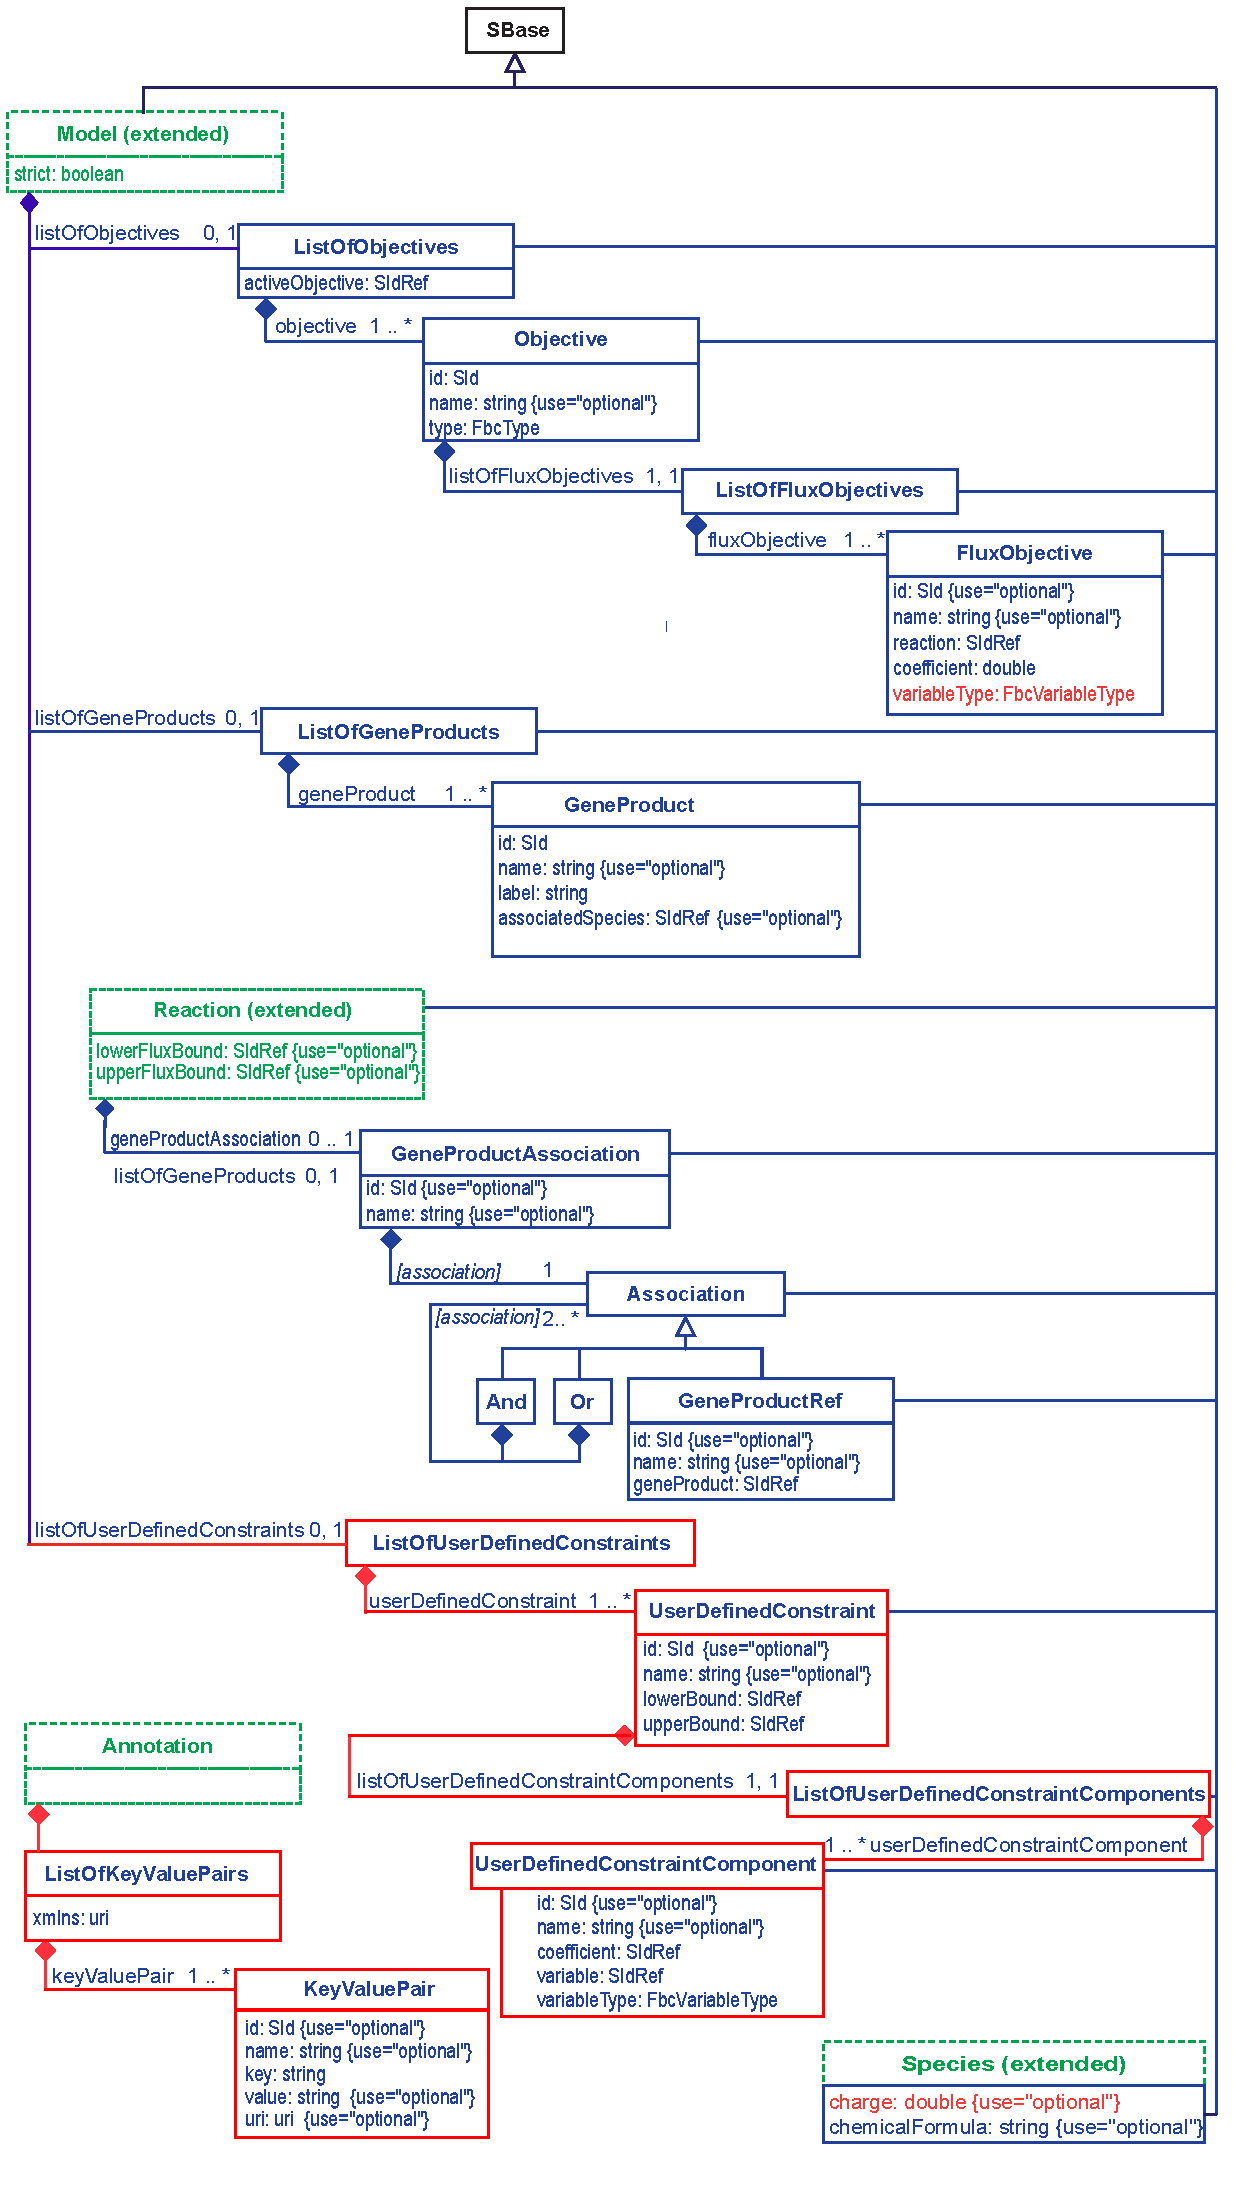
\includegraphics[height=0.85\textheight]{images/fbc_uml_v3.pdf}\\
  \caption{A UML representation of the \FBCPackage. Derived from \SBase, the
	\FBC classes inherit support for constructs such as SBML \Notes and
	\Annotation's. The [association] element name is the name of the class, de-capitalized.  In this case, the possible values are "and", "or", or "geneProductRef". See \ref{conventions} for conventions related to this figure.
	The individual classes are further discussed in the text.}
  \label{fig:fbc_uml}
\end{figure}



\subsection{Primitive data types}
\label{primtypes}

Section~3.1 of the \sbmlthreecore specification defines a number of primitive
data types and also uses a number of XML Schema 1.0 data types~\citep{biron:2000}.
More specifically we make use of \primtype{integer}, \primtype{double},
\primtype{string}, \primtype{SId} and \primtype{SIdRef}. In addition we make
use of a new primitive: the enumeration \primtype{FbcType}, see \ref{fig:fbc_uml}
for the interrelation between
these entities.

\newtxt{The \primtype{SId} type is used as the data type for the identifiers of \Objective (\ref{objective-class}), \FluxObjective (\ref{fluxobjective-class}), \GeneProduct (\ref{geneproduct-class}), \GeneProductAssociation (\ref{geneproductassociation-class}), \GeneProductRef (\ref{geneproductref-class}), \UserDefinedConstraint (\ref{userdefinedconstraint-class}), \UserDefinedConstraintComponent (\ref{userdefinedconstraintcomponent-class}) and \KeyValuePair (\ref{keyvaluepair-class}) classes.}
%
\newtxt{In all cases where the primitive data type \primtype{SId} is used in the \FBCPackage it is used unchanged from its description in \sbmlthreecore. When used as the type of a \token{fbc:id} attribute, that ID is added to the core \primtype{SId} namespace, and must continue to follow those rules for uniqueness: no \token{fbc:id} may duplicate any other \token{fbc:id}, nor the \token{id} of any \Model, \FunctionDefinition, \Compartment, \Species, \Reaction, \SpeciesReference, \ModifierSpeciesReference, \Event, or \Parameter, nor the \token{package:id} of any other SBML Level~3 package element that is also defined as being in the \primtype{SId} namespace.}

In the \FBCPackage the \ListOfObjectives has an attribute of type \primtype{SIdRef} that is used to
refer to an `active' \Objective as does the extended \Reaction class which defines two attributes referring to flux capacity constraints. The \GeneProductRef class declares an attribute of type \primtype{SIdRef} which references a \GeneProduct which itself contains an attribute that can refer to a \Species. \newtxt{Finally, the \UserDefinedConstraint and \UserDefinedConstraintComponent both declare attributes of type \primtype{SIdRef} and a more detailed description of what they refer to can be found in the relevant class descriptions.}

\subsubsection{Type \primtypeNC{FbcType}}
\label{primtype-fbctype}

The \FBCPackage defines a new enumerated type \primtype{FbcType} which represents the optimization sense of the objective function. It can have one of the following two values \val{maximize} or \val{minimize}.

\subsubsection{Type \primtypeNC{FbcVariableType}}
\label{primtype-fbcvariabletype}

\newtxt{The \FBCPackage defines a new enumerated type \primtype{FbcVariableType} which
represents the index of a variable that occurs in either the \FluxObjective or \UserDefinedConstraintComponent. It can have one of two values, \val{linear} or \val{quadratic}.}


\subsection{The extended \class{Model} class}
\label{model-class}
%\label{listoffluxbounds-class}

\newtxt{The \SBML \Model class is extended by adding a mandatory boolean attribute
\token{strict} as well as optional lists: \token{listOfObjectives}, \token{listOfGeneProducts} and \token{listOfUserDefinedConstraints}.} A \Model may contain, at most, one of each of these lists.

\begin{figure}[ht]
  \centering
  % Requires \usepackage{graphicx}
  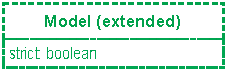
\includegraphics[width=6cm]{images/v3harmony_fbc_model.pdf}\\
  \caption{A UML representation of the extended \SBML \Model class used in
  the \FBCPackage. See \ref{conventions} for conventions related to this
  figure.}
  \label{fig:fbc_uml_model}
\end{figure}


%\begin{deprecated}
%\subsubsection{The \FBC \class{listOfFluxBounds}}
%
%As shown in \ref{fig:fbc_uml} the \ListOfFluxBounds is derived from \SBase
%and inherits the attributes \token{metaid} and \token{sboTerm}, as well as
%the subcomponents for \Annotation and \Notes. \ListOfFluxBounds must contain
%at least one \FluxBound (defined in \ref{fluxbound-class}).
%\end{deprecated}

\paragraph{The attribute \token{strict}}

The mandatory attribute \token{strict}, of type \primtype{boolean}, is used to apply an additional set of restrictions to the model. The \token{strict} attribute ensures that the \FBCPackage can be used to encode legacy FBA models expressible as Linear Programs (LP's) with software that is unable to analyze arbitrary mathematical expressions. In addition it ensures that a `strict' model is fully described and mathematically consistent, for example, by ensuring that all fluxes have a valid upper or lower bound.

\marginpar{\newtxt{How does strict interact with FBC3?}}

This is accomplished by defining a set of restrictions which come into effect if \token{strict} is set to \val{true}:
%
\begin{itemize}
	\item { Each \Reaction in a \Model must define attributes \token{lowerFluxBound} and \token{upperFluxBound} with each pointing to a valid \Parameter object defined in the current \Model.}
	\item {Each \Parameter object referred to by the \Reaction attributes \token{lowerFluxBound} and \token{upperFluxBound} must have their \token{constant} attribute set to \val{true} and its \token{value} attribute set to a \primtype{double} value which may not be \val{NaN}.
	}
	\item { \SpeciesReference elements of {\Reaction}s must have their \token{stoichiometry} attribute set to a \primtype{double} value that is neither \val{NaN} nor \val{-INF} nor \val{INF}. In addition their \token{constant} attribute must be set to \val{true}.
	}
	\item { \InitialAssignment elements may neither target the {\Parameter} elements referenced by the \Reaction attributes \token{lowerFluxBound} and
	        \token{upperFluxBound} nor any \SpeciesReference.
	}
	\item { All defined \FluxObjective elements must have their \token{coefficient} attribute set to a \primtype{double} value that is neither \val{NaN} nor \val{-INF} nor \val{INF}.
	}
	\item { A \Reaction \token{lowerFluxBound} attribute may not point to a \Parameter with a \token{value} of \val{INF}.}
	\item { A \Reaction \token{upperFluxBound} attribute may not point to a \Parameter with a \token{value} of \val{-INF}.}
    \item {For all reactions, the value of a \token{lowerFluxBound} must be less than or equal to the value of the \token{upperFluxBound}.}

\end{itemize}
%
While it is not compulsory for a `strict' \FBC model to define an \Objective, doing so does does allow it to be formulated as an LP and optimized, however, this decision is left to the modeler. Note that all other properties of the elements referred to in this list are as specified in the relevant \sbmlthreecore and \FBC specifications.

Alternatively, if the value of the \token{strict} attribute is \val{false} then none of these restrictions apply and the model creator can choose to define \FBC models that are not necessarily encodable as a LP. For example, if \token{strict} is \val{false} the \InitialAssignment construct may be used to set any valid numerical entity, including \Parameter values and stoichiometric coefficients, with any \primtype{double}. In addition, \Parameter elements are no longer required to be flagged as `constant' thus allowing for an \FBC model's use in alternative, hybrid modeling strategies.

\subsubsection{The \FBC \class{listOfObjectives}}
\label{listofobjectives-class}
As shown in \ref{fig:fbc_uml} the \ListOfObjectives is derived from \SBase
and inherits the attributes \token{metaid} and \token{sboTerm}, as well as
the subcomponents for \Annotation and \Notes. Unlike most other \SBML
\textsf{\textbf{ListOf\rule{0.15in}{0.5pt}}} classes, \ListOfObjectives
introduces an additional required attribute \token{activeObjective}. The
\ListOfObjectives must contain at least one \Objective (defined in
\ref{objective-class}).

\paragraph{The \token{activeObjective} attribute}
\label{activeObjective-attribute}

This attribute is of type \primtype{SIdRef} and can only refer to the
\token{id} of an existing \Objective. This required attribute exists
so that when multiple \Objective's are included in a single model, the
model will always be well described i.e., there is a single, primary
objective function which defines a single optimum and its associated
solution space.

\subsubsection{The \FBC \class{listOfGeneProducts}}
\label{listofgeneproducts-class}

As shown in \ref{fig:fbc_uml} the \ListOfGeneProducts is derived from \SBase
and inherits the attributes \token{metaid} and \token{sboTerm}, as well as
the subcomponents for \Annotation and \Notes. The \ListOfGeneProducts must
contain at least one \GeneProduct (defined in \ref{geneproduct-class}).

\subsubsection{The \FBC \class{listOfUserDefinedConstraints}}
\label{listofuserdefinedconstraints-class}

\newtxt{As shown in \ref{fig:fbc_uml} the \ListOfUserDefinedConstraints is derived from \SBase and inherits the attributes \token{metaid} and \token{sboTerm}, as well as the subcomponents for \Annotation and \Notes. The \ListOfUserDefinedConstraints must contain at least one \UserDefinedConstraint (defined in \ref{userdefinedconstraint-class}).}

\subsubsection{A note on units}
\label{fbcunits}
The main unit definitions that should be considered when using the \FBCPackage
are the global model definitions of ``extent''  and ``time'' as all \FBC flux
related classes (i.e., %\FluxBound and
\FluxObjective implicitly attains the same
unit as the \Reaction that they reference). More details on units can be found
in their respective class definitions.

\subsection{The extended \class{Species} class}
\label{species-class}

The \FBCPackage extends the \sbmlthreecore \Species class with the addition
of two attributes \token{charge} and \token{chemicalFormula}.
%
\begin{figure}[h]
  \centering
  % Requires \usepackage{graphicx}
  %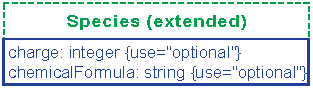
\includegraphics[width=6cm]{images/v2harmony_fbc_species.pdf}\\
  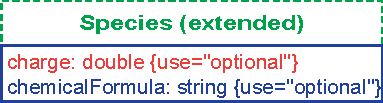
\includegraphics[width=6cm]{images/v3harmony_fbc_species.pdf}\\
  \caption{A UML representation of the extended \SBML \Species class used in
  the \FBCPackage. See \ref{conventions} for conventions related to this
  figure.}
  \label{fig:fbc_uml_species}
\end{figure}


%\paragraph{The \token{charge} attribute}
%The optional attribute \token{charge} which contains a signed
%\primtype{integer} referring to the \Species object's charge and is
%defined as it was in the \SBML Level 2 Version 1 specification
%: \textit{``The optional field charge takes an integer indicating
%the charge on the species (in terms of electrons, not the SI unit coulombs).''}
%
%\paragraph{The \token{chemicalFormula} attribute}
%\label{chemicalFormula-attribute}
%The optional attribute \token{chemicalFormula} containing a
%\primtype{string} that represents the \Species objects elemental
%composition.
%%
%\exampleFile{examples/ex_spec_l3.txt}
%%
%While there are many ways of referring to an elemental composition the purpose
%of the \token{chemicalFormula} attribute is to allow reaction balancing and
%validation which is particularly important in constraint-based models.
%
%The format of \token{chemicalFormula} must consist only of atomic names (as in
%the Periodic Table) or user defined compounds either of which take the form of
%a single capital letter followed by zero or more lowercase letters. Where there
%is more than a single atom present, this is indicated with an integer. With
%regards to order (and enhance inter-operability) it is recommended to use the
%Hill system order \citep{hillsystem, hillwikipedia}.
%
%%
%\begin{table}[h!]
%  %\centering
%  H2O4S\qquad C2H5Br\qquad BrH\\
%  C10H12N5O13P3\qquad CH3I\\
%  \caption{Examples of chemical formulas written using the Hill System. As
%	described in \ref{chemicalFormula-attribute}}\label{table:hill}
%\end{table}
%%
%Using this notation the number of carbon atoms in a molecule is indicated
%first, followed by the number of hydrogen atoms and then the number of all
%other chemical elements in alphabetical order. When the formula contains no
%carbon; all elements, including hydrogen, are listed alphabetically.

\paragraph{The \token{charge} attribute}

\newtxt{The optional attribute charge contains a signed double referring to the Species object’s charge (in terms of electrons, not the SI unit coulombs). Note, that unlike FBC versions one and two a \Species may, for the purposes of charge, be interpreted as a pseudoisomer or aggregate molecule and may assume a non-integer value. Non-integer charges should be used with caution as their use may have unintended side-effects, for example, with respect to the accuracy of reaction balancing.}

\paragraph{The \token{chemicalFormula} attribute}
\label{chemicalFormula-attribute}

The optional attribute \token{chemicalFormula} containing a \primtype{string} that represents the \Species objects elemental composition.

\newtxt{While there are many ways of referring to an elemental composition, the purpose of the \token{chemicalFormula} attribute is to enable reaction balancing and validation, something of particular importance in constraint-based models.}

\newtxt{The format of the \token{chemicalFormula} should, whenever possible, consist only of atomic names
(as in the Periodic Table). Similarly, for enhanced inter-operability, the element order should be arranged according to the Hill system (see \ref{table:hill2})} \citep{hillsystem, hillwikipedia}.
%
\begin{table}[h!]
  \begin{tabular}{ccc}
    % after \\: \hline or \cline{col1-col2} \cline{col3-col4} ...
     $H_{2}O_{4}S$ & $C_{2}H_{5}Br$ & $BrH$ \\
     $C_{10}H_{12}N_{5}O_{13}P_{3}$ & $CH_{3}I$ & $CH_{4}$  \\
  \end{tabular}
  \caption{Examples of chemical formulas written using the Hill System. As
	described in \ref{chemicalFormula-attribute}}\label{table:hill2}
\end{table}
%
\newtxt{Using this notation the number of carbon atoms in a molecule is indicated first, followed by the number of hydrogen atoms and then the number of all other chemical elements in alphabetical order. When the formula contains no carbon; all elements, including hydrogen, are listed alphabetically. Where there is more than a single atom present, this is indicated with an integer that follows the element symbol.}

\exampleFile{examples/ex-v3-species.txt}
%
\newtxt{However, in certain situations, it may become necessary to use a generic symbol to represent an undefined or generic component of a user-defined compound. Generic components can only be specified as the symbols \textsf{R} or \textsf{X}.}
%
\begin{table}[h!]
  \begin{tabular}{ccc}
    % after \\: \hline or \cline{col1-col2} \cline{col3-col4} ...
     $RCONH_{2}$ & $COX$ & $C_{2}H_{4}O_{2}(CH_{2})_{n}$ \\
  \end{tabular}
  \caption{Examples of chemical formulas written using the allowed non-Hill symbols described in \ref{chemicalFormula-attribute}.}\label{table:non-hill}
\end{table}
%
\newtxt{Furthermore, the undefined parenthesised group index $(\ldots)_n$ may also be used to indicate an arbitrary repetition of a chemical group. Note that a parenthesized group may only be followed by the subscript $n$. Integer values, for example, $(\ldots)_2$ and expressions such as $(\ldots)_{n-1}$ are considered invalid chemical formula.}

\newtxt{Please note, the use of \textsf{R}, \textsf{X} and $(\ldots)_n$ is not generally advised, as any \Reaction in which such a \Species occurs cannot necessarily be balanced and may lead to the construction of an invalid model. To highlight this potential problem, any \token{chemicalFormula} that contains any of the aforementioned, non-Hill compatible symbols will raise a `best practices' warning on model validation.}

\subsection{The \FBC \class{GeneProduct} class}
\label{geneproduct-class}
\GeneProduct is a new \FBC class derived from \SBML \SBase that inherits
\token{metaid} and \token{sboTerm}, as well as the subcomponents for
\Annotation and \Notes. The purpose of this class is to define a single gene
product. It implements two required attributes \token{id} and \token{label} as
well as two optional attributes \token{name} and \token{associatedSpecies}.

\begin{figure}[h]
  \centering
  % Requires \usepackage{graphicx}
  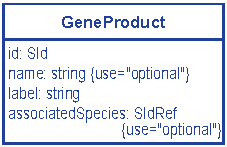
\includegraphics[width=5cm]{images/v2harmony_fbc_geneproduct.pdf}\\
  \caption{A UML representation of the \FBCPackage \GeneProduct class. For a complete description see \ref{fig:fbc_uml} as well as \ref{conventions} for conventions related to this figure.}
  \label{fig:fbc_uml_geneproduct}
\end{figure}

\paragraph{The \token{id} and \token{name} attributes}
A \GeneProduct has a required attribute \token{id} of type \primtype{SId}
and an optional attribute \token{name} of type \primtype{string}. The
unique \token{id} attribute is required to enable a \GeneProduct to be
referenced from a \GeneProductRef used in a \GeneProductAssociation.

\paragraph{The \token{label} attribute}
The primary purpose of a \GeneProduct is to uniquely reference a gene or
implied gene product. As there is, currently, no restriction on the format of these these references they cannot be assumed to conform to an \SBML \primtype{SId} syntax. Therefore the \FBCPackage defines the required attribute \token{label}, of type \primtype{string}, for this purpose.

%as seen in the example shown in \ref{intro-ga}
% % FB: taken out the sentence, as it does not add to the text
% As can be seen from the following examples, taken from existing models:
% \verb+Rv0649+, \verb+3074.1+ and \verb+CRv4_Au5.s2.g9153.t1+ there is
% currently no defined format for this gene identifier.
While ideally some form of restriction could, in principle, be placed on the value of \token{label}, at this point in time it is only possible to suggest that this attribute's value should conform to the definition of an
\primtype{SId}. For example, consider an existing GPR annotation, as encountered in legacy \SBML Level 2 encoded models:
\begin{verbatim}
 <p>GENE_ASSOCIATION: (Rv0649)</p>
\end{verbatim}
%
this can now be formally (and unambiguously) encoded as:
%
\exampleFile{examples/v2harmony-spec-example1-gene.txt}

Furthermore, it is a highly recommended `best practice' that a \GeneProduct be annotated using the inherited MIRIAM compliant \SBML \Annotation mechanism. Doing so will help reduce the dependence and ambiguity of using an overloaded, semantically meaningful \token{label} attribute and enhance interoperability. For an example of this approach see \ref{best-practices-cobraV2}.

\paragraph{The \token{associatedSpecies} attribute}
A \GeneProduct may, optionally, refer to a \Species so as to provide compatibility with the Manchester style encoding of gene-protein associations. In this case the attribute \token{associatedSpecies} is of type \primtype{SIdRef} and, if defined, must point to an existing \Species in the model.

%\begin{deprecated}
%\subsection{The \FBC \class{FluxBound} class}
%\label{fluxbound-class}
%
%\FluxBound is a new \FBC class derived from \SBML \SBase that inherits
%\token{metaid} and \token{sboTerm}, as well as the subcomponents for
%\Annotation and \Notes. The purpose of this class is to hold a single
%(in)equality that provides the maximum or minimum value that a reaction flux
%can obtain at steady state. It implements three attributes.
%
%Starting with Version~2 of the Flux Balance Constraints package the
%\FluxBound construct is deprecated. This is done to ease adoption and ensure that
%not all tools have to immediately implement support for changing flux bounds the
%attributes may also refer to the an existing \FluxBound in the model. However,
%that construct is deprecated and will be removed in a future version of this
%package.
%
%
%\begin{figure}[h!]
  %\centering
  %% Requires \usepackage{graphicx}
  %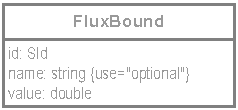
\includegraphics[width=5cm]{images/v2harmony_fbc_fluxbound.pdf}\\
  %\caption{A UML representation of the \FBCPackage \FluxBound class. See
  %\ref{conventions} for conventions related to this figure.}
  %\label{fig:fbc_uml_fbnd}
%\end{figure}
%
%\paragraph{The \token{id} and \token{name} attributes}
%A \FluxBound has the required attributes: \token{id} an attribute of type
%\primtype{SId} and an optional attribute \token{name} an attribute of type
%\primtype{string}.
%
%\paragraph{The \token{value} attribute}
%The \token{value} attribute holds a \primtype{double} value representing the
%numerical value of the flux bound. This may include an explicitly defined
%$\pm\infty$ encoded as a value, e.g., \val{INF}.
%
%For an example of the how the \FluxBound relates to the description of the
%underlying mathematical model please see \ref{examples1:fluxbound}.
%
%\paragraph{Units}
%The \token{value} defined by the \FluxBound has the units of the \token{reaction}
%that it refers to i.e.,~the globally defined unit of ``extent per time.''
%
%\paragraph{Reactions with undefined flux bounds}
%In the spirit of \sbmlthreecore the \FBCPackage does not define any default
%values for any element. However, in the case of a reaction with no defined
%flux bounds it is possible to infer this information from the reaction
%reversibility. In this case: irreversible reactions should be considered to
%be positive, $0 <= J <= \infty$ and reversible ones free/unbound,
%$-\infty <= J <= \infty$.
%
%Similarly, there is also the potential for a bound to ``seemingly'' conflict
%with the reaction that it bounds' reversibility, e.g., a reaction is
%irreversible but has bounds $-\infty <= J <= \infty$. In the context of
%this package, flux bounds should be considered authoritative. This follows
%from the fact that a \FluxBound can enforce an irreversible reaction, by
%restricting the flux ($0 <= J <= \infty$), as well as a reversible
%reaction ($-\infty <= J <= \infty$). It is left to the software
%implementation to deal with any obvious inconsistencies.
%
%\end{deprecated}

%\newpage

\subsection{The \FBC \class{Objective} class}
\label{objective-class}
\label{listoffluxobjectives-class}

The \FBC \Objective class is derived from \SBML \SBase and inherits
\token{metaid} and \token{sboTerm}, as well as the subcomponents for
\Annotation and \Notes. An integral component in a complete description
of a steady-state model is the so-called `objective function' which generally
consist of a linear combination of model variables (fluxes) and a sense
(direction). In the \FBC package this concept is succinctly captured in the
\Objective class.

\paragraph{The \token{id} and \token{name} attributes}
An \Objective has a required attribute \token{id} of type
\primtype{SId} and an optional attribute \token{name} of type \primtype{string}.

\paragraph{The \token{type} attribute}
The required \token{type} attribute contains an \primtype{FbcType} type
which represents the sense of the optimality constraint and can take one of
two values:
\begin{eqnarray*}
% I'm using \mapsto until I can find the proper symbol - bgoli
\label{obj-type-enum}
 \nonumber
  maximize & \mapsto & \textrm{``}\mathtt{maximize}\textrm{''}\\
  minimize & \mapsto & \textrm{``}\mathtt{minimize}\textrm{''}
\end{eqnarray*}

\paragraph{The \token{listOfFluxObjectives} element}
The element \token{listOfFluxObjectives} which contains a
\ListOfFluxObjectives is derived from and functions like a typical \SBML
\textsf{\textbf{ListOf\rule{0.15in}{0.5pt}}} class with the restriction that it
must contain one or more elements of type \FluxObjective (see \ref{fluxobjective-class}).
This implies that if an \Objective is defined there should be at least
one \FluxObjective contained in a \ListOfFluxObjectives.
% bgoli: to me this makes sense but are there other examples of this in SBML or is everything always optional

\begin{figure}[ht]
  \centering
  % Requires \usepackage{graphicx}
  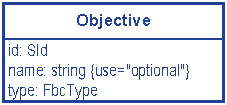
\includegraphics[width=5cm]{images/v2harmony_fbc_objective.pdf}\\
  \caption{A UML representation of the \FBCPackage \Objective class. For a complete description see \ref{fig:fbc_uml} as well as \ref{conventions} for conventions related to this figure.}
  \label{fig:fbc_uml_obj}
\end{figure}

\pagebreak
\paragraph{Encoding the \Objective}
The \FBCPackage allows for the definition of multiple model objectives with
one being designated as active (see \ref{objective-class}) as illustrated in
this example:
%
\exampleFile{examples/ex_objf_fbc.txt}
%
Note how both \Objective instances differ in \token{type} and each contains
different set of \class{FluxObjectives} (see \ref{fluxobjective-class}).
For an example of how the \Objective relates to the description of the
underlying mathematical model please see \ref{examples1:objfunc}.

%\subsection{The \FBC \class{FluxObjective} class}
%\label{fluxobjective-class}
%
%The \FBC \FluxObjective class is derived from \SBML \SBase and inherits
%\token{metaid} and \token{sboTerm}, as well as the subcomponents for
%\Annotation and \Notes.
%
%The \FluxObjective class is a relatively simple container for a model
%variable weighted by a signed linear coefficient.
%
%%
%\begin{figure}[ht]
%  \centering
%  % Requires \usepackage{graphicx}
%  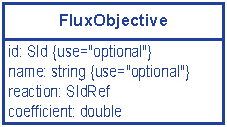
\includegraphics[width=5cm]{images/v2harmony_fbc_fluxobjective.pdf}\\
%  \caption{A UML representation of the \FBCPackage \FluxObjective class. For a complete description see \ref{fig:fbc_uml} as well as \ref{conventions} for conventions related to this figure.}
%  \label{fig:fbc_uml_fobj}
%\end{figure}
%
%\paragraph{The \token{id} and \token{name} attributes}
%A \FluxObjective has two optional attributes: \token{id} an attribute of
%type \primtype{SId} and \token{name} an attribute of type \primtype{string}.
%
%\paragraph{The \token{reaction} and \token{coefficient} attributes}
%The required \token{reaction} is of type \primtype{SIdRef} and is restricted
%to refer only to a \Reaction while the \token{coefficient} attribute
%holds a \primtype{double} referring to the coefficient that this \FluxObjective
%takes in the enclosing \Objective. For example the objective
%\texttt{ Maximize: 1 R1 + 2 R2} would be encoded as
%%
%\exampleFile{examples/ex_fluxobj_fbc.txt}
%
%\paragraph{Units}
%As described above the \FluxObjective defined here as $n\cdot J$ where
%the \token{coefficient} ($n$) is dimensionless and the \token{value} ($J$)
%takes the units of the \token{reaction} flux i.e.,~``extent per time''.
%Therefore, the \FluxObjective ($n\cdot J$)  has the unit ``extent per time''
%where the units of reaction ``extent'' and ``time'' are defined globally.

\subsection{The \FBC \class{FluxObjective} class}
\label{fluxobjective-class}

The \FBC \FluxObjective class is derived from \SBML \SBase and inherits \token{metaid} and \token{sboTerm}, as well as the subcomponents for \Annotation and \Notes.
%
\newtxt{The FluxObjective class is a relatively simple container for a model variable weighted by a signed numerical coefficient. The model variable is defined as being either a `linear' or `quadratic' variable.}
%
\begin{figure}[ht]
  \centering
  % Requires \usepackage{graphicx}
  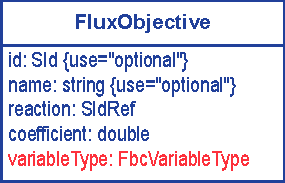
\includegraphics[width=6cm]{images/fbc_v3_uml_fobj.pdf}\\
  \caption{A UML representation of the \FBCPackage \FluxObjective class. For a complete description see \ref{fig:fbc_uml} as well as \ref{conventions} for conventions related to this figure.}
  \label{fig:fbc_uml_userdefinedconstraint}
\end{figure}
%
% I don't thing this is needed
%\newtxt{The \FluxObjective class is a relatively simple container for a model variable that can be defined as the variable type `linear' or `quadratic' and weighted by a signed linear coefficient.}
%
\paragraph{The \token{id} and \token{name} attributes}
A \FluxObjective has two optional attributes: \token{id} an attribute of
type \primtype{SId} and \token{name} an attribute of type \primtype{string}.

\paragraph{The \token{reaction} and \token{coefficient} attributes}
The required \token{reaction} is of type \primtype{SIdRef} and is restricted
to refer only to a \Reaction while the \token{coefficient} attribute
holds a \primtype{double} referring to the coefficient that this \FluxObjective
takes in the enclosing \Objective expression.

\newtxt{\paragraph{The \token{variableType} attribute}
The required \token{variableType} attribute contains a \primtype{FbcVariableType} that
represents the index to which a variable is raised in a \FluxObjective. For example, where $J$ represents a steady-state flux the \primtype{FbcVariableType} defines either a \val{linear}, $J^1$ or \val{quadratic}, $J^2$ term.}

\paragraph{Two examples of objective functions encoded in \SBML}
\newtxt{A common linear objective function (expressed in LP format):} \verb"Maximize: 1 R1"
%
\exampleFile{examples/ex-v3-fluxobjective-linear.txt}
%
\newtxt{An advanced objective function with both a linear and quadratic term (expressed in LP format):} \verb"Minimize: 1 R1 + [4 R2^2]/2"
%
\exampleFile{examples/ex-v3-fluxobjective.txt}

\paragraph{Units}
As described above the linear \FluxObjective defined here as $n\cdot J$ where
the \token{coefficient} ($n$) is dimensionless and the \token{value} ($J$)
takes the units of the \token{reaction} flux i.e.,~``extent per time''.
\newtxt{Therefore, the \token{linear} \FluxObjective, ($n\cdot J$)  has the unit $\frac{extent}{time}$ where the units of reaction ``extent'' and ``time'' are defined globally. Analogously, in the case of a \token{quadratic} \FluxObjective, $n\cdot J^{2}$ this would be $\frac{extent^{2}}{time^{2}}$}.

